\subsection{Life cycle of a Crawler module}

Upon launch, Launcher parses the command line. It decides that a Crawler must
be started. This will read the parameters stored in Psyclone. The available parameter names are:

\begin{itemize}
 \item[OPML] URL to a OPML file containing URLs to RSS feeds.
 \item[RSS] URL to a RSS feed. Only read if the OPML parameter is unavailable.
 \item[RefreshTime] The time in seconds between feed refreshes.
\end{itemize}

The crawler will then create the appropriate channels and starts polling them
in an infinite loop (of course with some time between two polls).

\begin{figure}[htp]
  \centering
  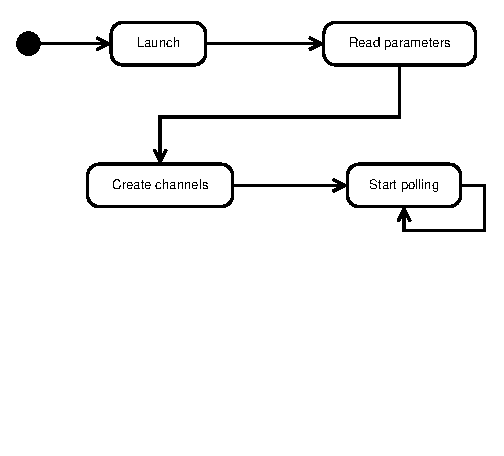
\includegraphics{image/sequence-diagram-crawler}
  \caption{Sequence diagram of a Crawler module}
\end{figure}
